

\section{\we Framework}

Motivated by the observations in Section~\ref{sec:motivation}, we design \we to decouple historical-context modeling from speculative generation. As illustrated in Figure~\ref{fig:background}(e), instead of requiring a lightweight draft model to repeatedly process and maintain an ever-growing history, \we delegates global-context modeling to the target model and performs drafting only over compact target hidden states. This design transforms speculative drafting \textbf{from an increasingly complex growing-history modeling problem into a local prediction problem} whose structure and positional range remain independent of the accumulated sequence length. \we realizes this principle through a history-free semi-autoregressive architecture and a two-stage training strategy.

% v2
% Motivated by the findings in Section~\ref{sec:motivation}, \we decouples historical-context modeling from speculative generation. The target model remains responsible for processing the complete context, while the draft model operates only on compact target representations and a sliding anchor group. \we consists of two key components: a history-free semi-autoregressive architecture for efficient speculative generation and a two-stage training strategy for effectively training the history-free drafter.


% v1
% The key design principle of \we is to avoid repeatedly encoding and maintaining the complete historical context within the draft model. Instead, \we directly reuses contextual hidden states produced by the target model and performs speculation only over a sliding anchor group. To achieve both high drafting quality and low execution overhead, \we is built upon a history-free semi-autoregressive architecture in Section~\ref{sec:DLite:arch} and is further trained through the specific two-stage strategy in Section~\ref{sec:DLite:train}. 
% In the following, we first introduce the History-Free Semi-Autoregressive Architecture, followed by the Two-Stage Training Strategy.


\subsection{History-free semi-autoregressive Architecture} \label{sec:DLite:arch}

Figure~\ref{fig:overview} illustrates the inference dataflow of \we. The target model first processes the input context and maintains its original KV cache. For each speculative round, \we takes contextual hidden states from the target model, the current anchor token, and \(K\) draft placeholders as input. A history-free parallel backbone produces hidden representations for all speculative positions simultaneously, after which a lightweight sequential head restores the causal dependency among tokens within the speculative block. The resulting candidate tokens are finally verified by the target model following the standard speculative decoding procedure. It is worth noting that \we maintains no historical draft KV cache throughout this process. Each speculative round is independently reconstructed from the latest target representations and the current anchor token, allowing the drafter to perform prediction locally without explicitly processing the accumulated history.


% v2
% Figure~\ref{fig:overview} illustrates the inference workflow of \we. The target model first processes the input context and maintains its original KV cache. For each speculative round, \we takes target hidden states, a small sliding anchor group, and \(K\) draft placeholders as input. A history-free parallel backbone produces hidden representations for all speculative positions simultaneously, after which a lightweight sequential head restores the causal dependency among tokens within the speculative block. The resulting draft tokens are finally verified by the target model in the standard speculative-decoding pipeline. It is worth noting that, unlike conventional drafters, \we maintains no historical draft KV cache throughout this process.

% v1
% Figure~\ref{fig:overview} illustrates the overall inference workflow and architecture of \we. \we adopts a history-free semi-autoregressive design that directly reuses contextual representations produced by the target model, instead of maintaining an independent historical KV cache for the draft model. The architecture consists of two components: \textbf{a history-free parallel backbone} and \textbf{a lightweight sequential head}.

% Given an input prompt, the target model first performs standard prefill operation and maintains its original KV cache. The parallel backbone then takes hidden states extracted from the target model, the sliding anchor group, and several draft placeholders as input, and produces hidden states for multiple speculative positions in parallel. A lightweight sequential head further introduces causal dependencies among the speculative tokens before they are verified by the target model. During this process, \we will \textbf{not} store any historical KV cache.

\begin{figure}[!t]
    \centering
    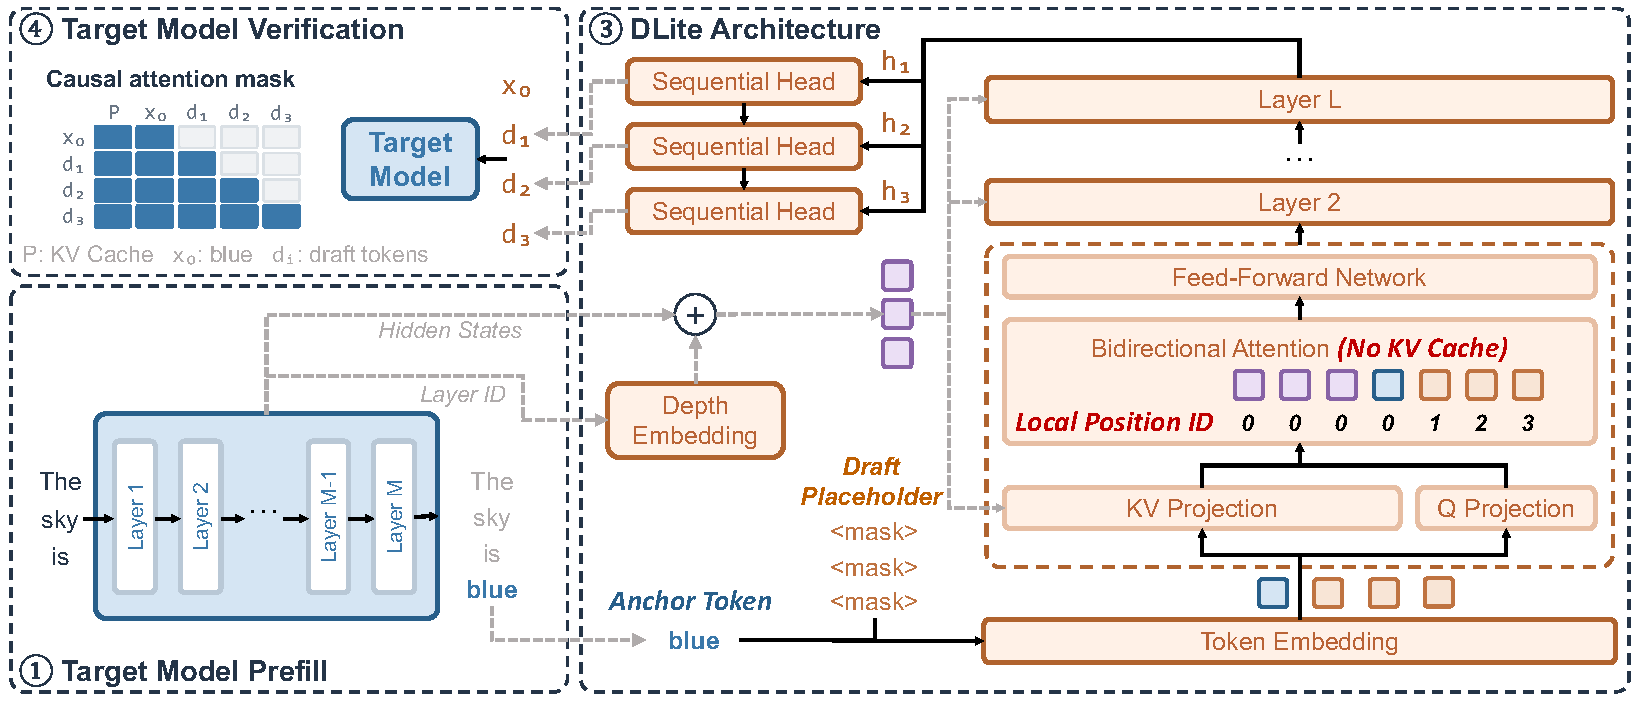
\includegraphics[width=0.98\textwidth]{fig/overview2.pdf}
    \vspace{-5pt}
    \caption{The inference dataflow of \we.}
    \label{fig:overview}
    \vspace{-10pt}
\end{figure} 

\subsubsection{History-free Parallel Backbone}

The key idea of the history-free parallel backbone is to \textbf{transform speculative drafting from growing-history modeling into local prediction}. To this end, the backbone combines compact target hidden states with explicit local token information and performs local prediction.


% v2
% The parallel backbone is designed to extract sufficient contextual information for speculation without independently reconstructing the full historical context. It combines three sources of information: target hidden states, a sliding anchor group, and local positional information.


\textbf{Target hidden states.} \we directly reuses hidden states produced by the target model as compact contextual features. Since target hidden states and ordinary token embeddings correspond to different input sources, we introduce a learnable depth embedding to distinguish them. When hidden states from multiple target layers are used, the same embedding also identifies their source layers. For a target hidden state \(h_t^{(l)}\) extracted from layer \(l\), we construct
\begin{equation}
    z_t^{(l)} = h_t^{(l)} + e_{\mathrm{depth}}^{(l)}
\end{equation}
where \(e_{\mathrm{depth}}^{(l)}\) is a learnable source-specific embedding.

% \textbf{Sliding anchor group.} Target hidden states provide a compact representation of the historical context, but may lose fine-grained information about the most recent tokens. \we therefore retains a small sliding anchor group around the current decoding position to provide explicit local token information. As decoding proceeds, the anchor group moves forward with the accepted prefix. Its size remains fixed, allowing the backbone to preserve fine-grained short-range context without introducing a growing historical state.


\textbf{Local prediction.} Conventional drafters operate over an ever-growing history, such that both the explicit context and global positions increase as decoding proceeds. \we instead delegates long-context modeling to the target model and performs draft prediction only around the current decoding position. The backbone takes the current anchor token and \(K\) speculative positions, while using local rather than globally accumulated positions. Historical information is retained through the target hidden states, allowing the drafter to focus on local prediction without explicitly reconstructing the history. \we therefore transforms growing-history modeling into a local prediction problem. 

% \textbf{Fixed-size local prediction.} Conventional speculative drafters operate on an ever-growing historical sequence. At decoding position \(t\), the drafter must predict future tokens conditioned on $x_{<t}$ whose length and associated global positions continuously increase as decoding proceeds. For a lightweight draft model, the structure of the prediction problem therefore becomes increasingly demanding as the historical context grows. 

% \we removes this dependence by delegating long-context hidden states to the target model. Given the compressed target hidden states and a fixed-size anchor group of size \(A\), the draft backbone only operates over a local prediction window containing \(A\) anchor tokens and \(K\) speculative positions. Accordingly, \we assigns positions relative to the current local window rather than using globally accumulated positions. The positional range is always

% \begin{equation}
%  \{0,1,\ldots,A+K-1\}
% \end{equation}

% regardless of whether the original sequence contains thousands or hundreds of thousands of tokens.

% Therefore, as the sequence grows, the structural complexity of the draft-side prediction problem remains bounded: both the explicit token context and positional range seen by the backbone remain fixed. \we thus converts an increasingly long-context prediction problem into \textbf{a fixed-size local prediction problem that is independent of the accumulated sequence length}.

% Each speculative round is consequently reconstructed from the current target hidden states, sliding anchors, and draft placeholders without caching historical backbone states. Formally, given the target features \(\mathcal{Z}_t\), anchor group \(A_t\), and \(K\) draft placeholders \(M_{1:K}\), the parallel backbone produces

% \begin{equation}
% (h_1,h_2,\ldots,h_K) = F_{\theta} \left( \mathcal{Z}_t, A_t, M_{1:K} \right)
% \end{equation}

% where \(h_T\) denotes the hidden states corresponding to the \(T\)-th speculative position. All \(K\) representations are computed in parallel using bidirectional attention within the local window.


% v2
% \textbf{History-free computation and local positions.} Unlike conventional speculative drafters, \we does not cache any historical backbone states. Each speculative round is reconstructed from the current target hidden states, sliding anchors, and draft placeholders. Therefore, the draft-side state does not grow with the accumulated sequence history.

% To match this history-free computation, \we uses local position embeddings within the current speculative window rather than globally accumulated sequence positions. Positions are defined only relative to the local anchor-and-draft window, so each speculative round is formulated as a fixed-size local prediction problem independent of the absolute sequence position.

% Given the target features \(\mathcal{Z}_t\), anchor group \(A_t\), and \(K\) draft placeholders \(M_{1:K}\), the parallel backbone produces
% \begin{equation}
%     (h_1,h_2,\ldots,h_K) = F_{\theta} \left( \mathcal{Z}_t, A_t, M_{1:K} \right) 
% \end{equation}
% where \(h_T\) denotes the backbone representation for the \(T\)-th speculative position.


% The history-free parallel backbone is the core component that enables \we to perform efficient speculative drafting without maintaining a historical KV cache. Its design is built on four key ideas: depth-aware target features, a sliding anchor group, history-free computation without KV cache, and local position encoding.

% First, \we directly reuses hidden states from the target model as compact contextual inputs. Since hidden representations from different target layers capture complementary semantic information, \we introduces a learnable depth embedding to encode the source-layer identity of each extracted hidden state. Specifically, for the hidden state \(h_t^{(l)}\) taken from target layer \(l\), we construct a depth-aware feature as
% \begin{equation}
%     z_t^{(l)} = h_t^{(l)} + e_{\mathrm{depth}}^{(l)}
% \end{equation}

% where \(e_{\mathrm{depth}}^{(l)}\) is a learnable source-specific embedding. This embedding allows the backbone to distinguish token embeddings from target hidden states and, when multiple target layers are used, to distinguish hidden states originating from different depths, rather than treating all inputs as homogeneous representations.

% Second, \we introduces a sliding anchor group composed of a small number of recent tokens near the current decoding position. While the target hidden states provide a compressed representation of the full historical context, the anchor group preserves fine-grained local token information that is especially useful for short-range continuation. As decoding proceeds, this anchor group slides forward with the accepted prefix, ensuring that the backbone always conditions on the most relevant local context while keeping the input length fixed.

% Third, unlike conventional speculative drafters, the \we backbone performs history-free computation without maintaining any draft KV cache. Existing methods typically preserve historical draft states and incrementally update them after each verification step, which incurs additional synchronization and maintenance overhead. In contrast, \we reconstructs each speculative round from scratch using only the current target features, the sliding anchor group, and several draft placeholders. As a result, the computational and memory cost of the backbone is independent of the accumulated decoding history.

% Finally, to match this history-free design, \we adopts local position embeddings within the current speculative window, rather than absolute or globally accumulated positions over the full sequence. The anchor tokens and speculative placeholders are assigned positions only relative to the current local window. This local position scheme allows the backbone to focus on short-range structural relationships among the anchor group and speculative positions, while avoiding any dependence on the absolute sequence length. It also naturally aligns with the no-KV-cache design, since each speculative round is computed as an independent local prediction problem.

% Based on these designs, the backbone takes as input the depth-aware target features, the sliding anchor group, and the draft placeholders, and applies bidirectional attention to produce hidden representations for all speculative positions in parallel:

% $$ h_1, h_2, \ldots, h_K . $$

% These representations summarize both the global contextual information extracted from the target model and the local structural information encoded within the speculative window, and are then passed to the lightweight sequential head for causal refinement.


\subsubsection{Lightweight Sequential Head}


While the parallel backbone efficiently produces representations for multiple speculative positions, parallel computation removes the autoregressive dependency among tokens within the speculative block. \we therefore introduces a lightweight sequential head that \textbf{restores only the missing intra-block dependency}, rather than performing another full contextual modeling process.


Let \(t\) denote the starting position of a speculative block and \(T\) the intra-block offset. The target model predicts \(x_{t+T}\) autoregressively according to
\begin{equation}
p_T \left( x_{t+T}\mid x_{<t+T} \right) = p_T \left( x_{t+T} \mid x_{<t}, x_{t:t+T-1} \right) 
\end{equation}
The parallel backbone, however, produces \(h_T\) before the tokens at earlier speculative positions are sampled. Since the preceding context \(x_{<t}\) has already been processed by the target model and conveyed through its contextual representations into \(h_T\), the information missing from parallel drafting is precisely the intra-block prefix $ x_{t:t+T-1}$. This decomposition suggests that the sequential module does not need to reconstruct the complete historical context. It only needs to encode tokens generated earlier within the current speculative block.

To recover this missing dependency efficiently, we employ a low-rank RNN-style sequential head. It recursively compresses previously generated draft tokens into a recurrent state
\begin{equation}
s_T = g_{\phi} \left( s_{T-1}, E(x_{t+T-1}) \right)
\end{equation}
where \(E(\cdot)\) denotes the token embedding. The prediction at speculative position \(T\) is modeled as
\begin{equation}
q_{\theta,\phi} \left( x_{t+T}\mid h_T,s_T \right) \approx p_T \left( x_{t+T} \mid x_{<t}, x_{t:t+T-1} \right)
\end{equation}
Here, \(h_T\) supplies the contextual information already encoded by the target model, while \(s_T\) summarizes the missing intra-block prefix. Together, they recover the information required for autoregressive prediction without reconstructing the full history inside the draft model. This preserves most contextual computation in the parallel backbone while restricting sequential execution to a lightweight low-rank module.

Furthermore, unlike existing semi-autoregressive methods that first project every backbone representation into full-vocabulary logits and subsequently refine these predictions with an additional sequential module, \we performs sequential modeling directly in the hidden space. The vocabulary projection is applied only after the intra-block dependency has been incorporated.

For hidden dimension \(D\) and vocabulary size \(V\), this avoids repeatedly applying an intermediate \(D\times V\) projection to every speculative representation before sequential refinement. Such computation becomes particularly expensive under high-concurrency serving, where a large number of speculative hidden states are processed simultaneously.



% v2
% Parallel drafting reduces draft latency by predicting multiple speculative positions simultaneously. However, this parallelism removes the auto-regressive dependency among speculative positions, causing prediction quality to degrade at deeper draft positions. As observed by DSpark, explicitly restoring \textbf{intra-block sequential dependency} is important for maintaining high acceptance rates. Following this insight, we introduce a sequential decoding stage on top of the parallel backbone. Unlike existing methods that first project each backbone hidden state into full-vocabulary logits and then employ an additional sequential head to refine these predictions, we find that the expensive vocabulary projection is unnecessary for draft prediction.

% Let $t$ denote the starting position of a speculative block and $T$ denote the intra-block offset. The target model predicts \(x_{t+T}\) auto regressively according to $p(x_{t+T} \mid x_{<t}, x_{t:t+T-1})$. In contrast, the parallel backbone produces a hidden representation $h_T$ without observing the tokens sampled at earlier positions within the same block. In \we, the preceding context \(x_{<t}\) is compactly conveyed through the target representation \(H_t\) and encoded into \(h_T\). To align with the target model’s auto-regressive formulation, the missing information in parallel drafting is precisely the intra-block prefix token \(x_{t:t+T-1}\).

% To efficiently recover this missing dependency, we employ a low-rank RNN-style head that recursively compresses previously generated draft tokens within the draft block into a recurrent state: 
% $s_T = RNN(s_{T-1}, x_{t+T-1})$. 
% The prediction at position \(T\) is then directly modeled as
% $ q_\theta(x_{t+T}\mid h_T,s_T) \approx p(x_{t+T}\mid x_{<t},x_{t:t+T-1}).$ Here, \(s_T\) summarizes the intra-block prefix. Together, they recover the information required for autoregressive prediction.

% This formulation also avoids the expensive intermediate vocabulary projection used by existing sequential-refinement methods. Instead of first projecting each \(D\)-dimensional backbone hidden state into \(V\)-dimensional logits and then refining these logits with an additional sequential module, \we restores the missing sequential dependency directly in the low-rank hidden space. This is particularly important for high-concurrency serving, where repeatedly applying a \(D\times V\) vocabulary projection to a large batch of speculative hidden states can become a significant drafting bottleneck. 

% In Exp Section, Our method can reduce the draft latency by 70\%, leading to 10\% - 20\% throughput improvement under multi-request scenario.



\begin{figure}[!t]
    \centering
    \vspace{-12pt}
    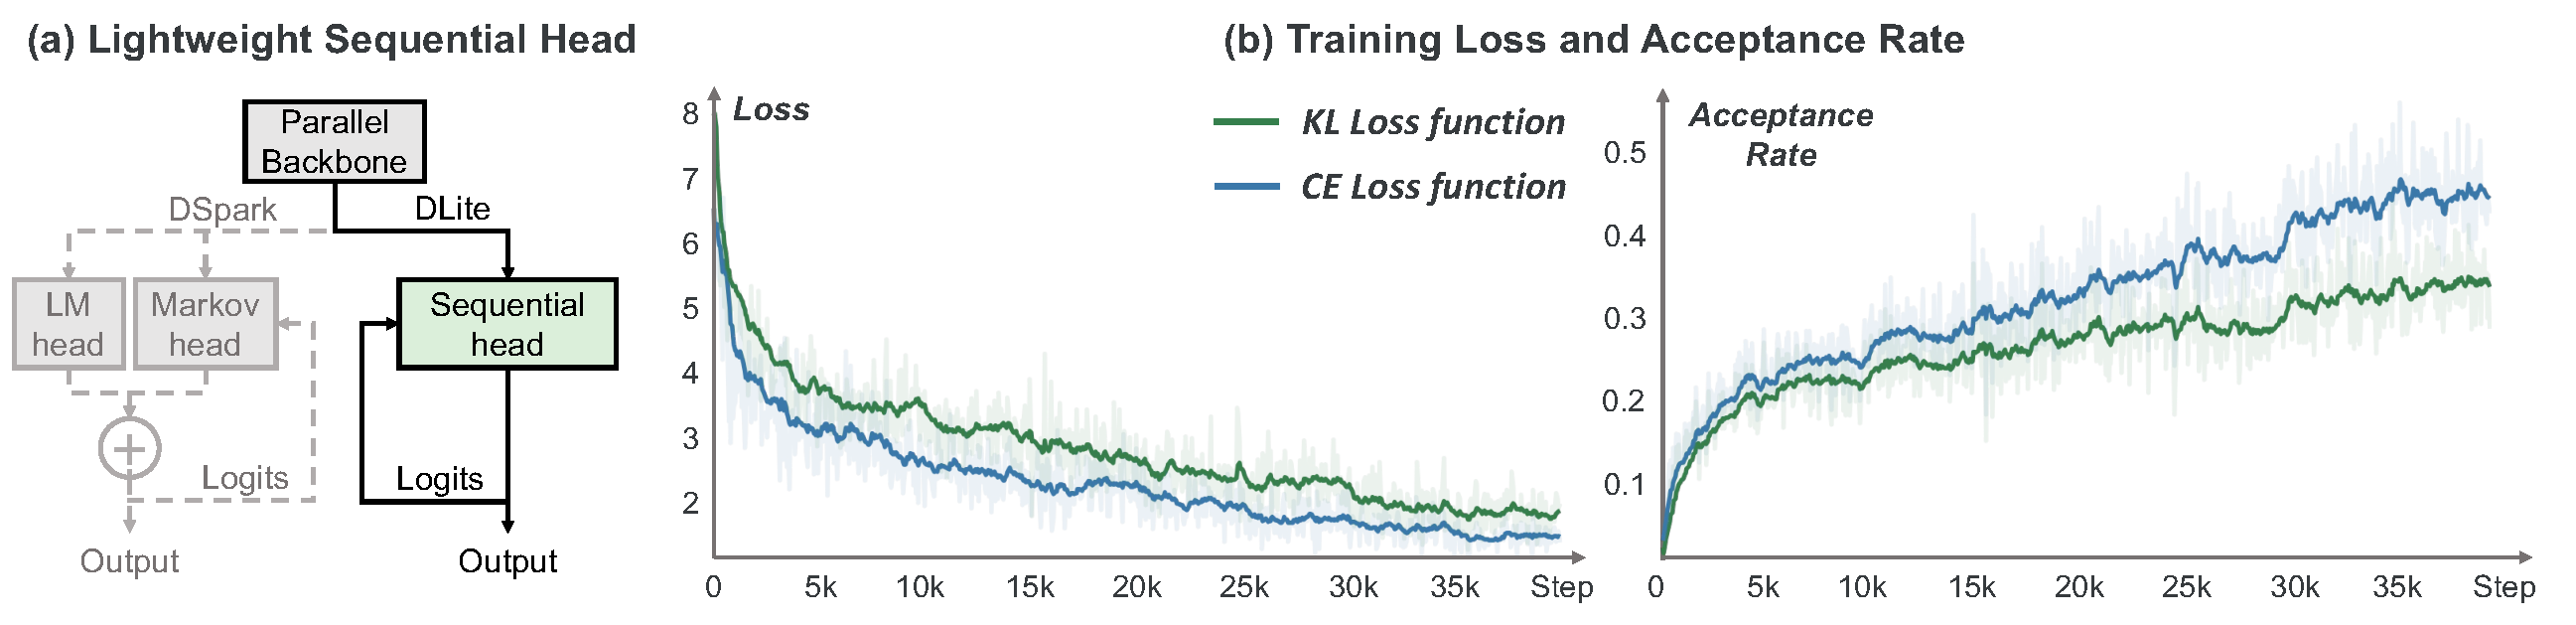
\includegraphics[width=\linewidth]{fig/training.pdf}
    \caption{(a) The design architecture of the lightweight sequential head. (b) The training loss and acceptance rate curves of direct target-model distillation using KL and CE loss function.}
    \label{fig:train}
    \vspace{-15pt}
\end{figure}


\subsection{Two-stage Training Strategy} \label{sec:DLite:train}
The objective of a speculative draft model is to approximate the predictive distribution of the target model, since a larger distribution overlap generally leads to a higher speculative acceptance probability. Distribution-level objectives such as KL divergence are therefore natural choices for distillation. However, Figure~\ref{fig:train}(b) shows that directly applying KL distillation from the target model to the parallel backbone in \we performs poorly. The two models make predictions under substantially different conditions: the target model performs autoregressive prediction over the complete historical context, whereas the backbone performs parallel prediction using compressed target hidden states,
% Consequently, their output distributions are induced by heterogeneous prediction structures and conditioning information, 
making direct distribution alignment difficult. To bridge this structural gap, we introduce a two-stage training strategy. The warm-up stage first trains \we against an isomorphic history-aware teacher, providing a structurally matched intermediate distillation target. The stable stage subsequently removes this teacher and directly aligns \we with the original target model. Let \(K\) denote the speculative block length and \(V\) the vocabulary size. At speculative position \(i\), we denote the predictive distributions of the target model, history-aware teacher, and \we as $p_i^T, p_i^H, q_i$ respectively, and denote the ground-truth token as \(y_i\).


% v2
% The ultimate objective of a speculative draft model is to approximate the predictive distribution of the target model, since a larger overlap between the two distributions generally leads to a higher acceptance probability. Compared with hard-label cross-entropy, which only supervises the probability assigned to the observed token, KL divergence provides dense supervision over the entire target distribution and is therefore a natural objective for distribution-level distillation. However, Figure~\ref{fig:train}(b) shows that directly applying KL distillation between \we and the target model performs poorly in our experiments. We attribute this difficulty to the substantial mismatch between their prediction structures and conditioning information: the target model performs autoregressive prediction over the complete historical context, whereas \we performs history-free block prediction using compressed target features and local tokens. Consequently, the two distributions are induced under heterogeneous prediction conditions, making direct distribution alignment difficult.

% To effectively exploit distribution-level supervision while addressing this structural mismatch, we introduce a two-stage training strategy. The first stage constructs a history-aware model that is architecturally aligned with \we and uses it as an intermediate teacher for KL distillation. The second stage removes this intermediate teacher and directly aligns \we with the original target model using objectives that are better aligned with speculative acceptance.

% Let \(K\) denote the speculative block length and \(\mathcal{V}\) the vocabulary. For the \(i\)-th speculative position, we denote the output distributions of the target model, the history-aware teacher, and \we as \(p_i^{T}\), \(p_i^{H}\), and \(q_i\), respectively, and denote the supervision token as \(y_i\).



% \subsubsection{Warm-up Stage}


\textbf{Warm-up Stage.} In the warm-up stage, we first train an isomorphic history-aware teacher by standard token-level cross-entropy (\(-\sum_i w_i \ \mathrm{log}\ {p_i^H(y_i)}\)). The teacher shares the same backbone and prediction structure as \we, but retains access to historical KV cache. 
% Since this teacher does not need to learn history-free prediction from the beginning, it can be effectively optimized with .
% \[
% \mathcal{L}_{\mathrm{teacher}}
% =
% \mathcal{L}_{\mathrm{CE}}
% =
% -\frac{1}{K}
% \sum_{i=1}^{K}
% \log p_i^{H}(y_i).
% \]
Once the history-aware teacher is sufficiently trained, we use it as an intermediate distillation target for \we using forward KL divergence: 
\begin{equation}
\mathcal{L}_{\mathrm{warmup}}
=
\sum_{i=1}^{K}
w_i D_{\mathrm{KL}}
\left(
p_i^{H}\,\|\,q_i
\right)
=
\sum_{i=1}^{K}
w_i
\sum_{v\in\mathcal V}
p_i^{H}(v)
\log
\frac{p_i^{H}(v)}
{q_i(v)}
\end{equation}
where \(w_i = \exp(\frac{-(i-1)}{\gamma})\) emphasizes the contribution of earlier positions. Because the teacher and \we share the same architecture and prediction interface, their output distributions are naturally aligned despite the difference in historical information available to them.

The history-aware teacher therefore serves as an optimization bridge between the autoregressive target model and the history-free drafter. Instead of forcing \we to directly match a target distribution, the warm-up stage first exposes it to a structurally matched predictive distribution, providing a more stable starting point for subsequent target-model alignment.


%v2
% In the warmup stage, we first train an isomorphic history-aware teacher that shares the same backbone and prediction structure as \we, but retains access to historical KV cache. Since this teacher does not need to learn history-free prediction from the beginning, it can be effectively optimized with standard token-level cross-entropy:
% \[
% \mathcal{L}_{\mathrm{teacher}}
% =
% \mathcal{L}_{\mathrm{CE}}
% =
% -\frac{1}{K}
% \sum_{i=1}^{K}
% \log p_i^{H}(y_i).
% \]Once the history-aware teacher is sufficiently trained, we use it as an intermediate distillation target for \we. Because the teacher and \we share the same architecture and prediction interface, their output distributions are naturally aligned despite the difference in historical information available to them. We therefore optimize \we using forward KL divergence:
% \[
% \mathcal{L}_{\mathrm{warmup}}
% =
% \frac{1}{K}
% \sum_{i=1}^{K}
% D_{\mathrm{KL}}
% \left(
% p_i^{H}\,\|\,q_i
% \right)
% =
% \frac{1}{K}
% \sum_{v\in\mathcal V}
% p_i^{H}(v)
% \log
% \frac{p_i^{H}(v)}
% {q_i(v)}.
% \]Instead of forcing the history-free model to directly match the substantially different target model from the beginning, this stage uses the history-aware isomorphic teacher as an optimization bridge, guiding \we toward a stable parameter region while progressively transferring the predictive capability obtained from historical context into the history-free architecture.


% \subsubsection{Stable Stage}


\textbf{Stable Stage.} Although the intermediate teacher facilitates optimization, the ultimate objective of \we is to match the predictive distribution of the target model. We therefore discard the history-aware teacher 
in the stable stage and directly optimize \we against the target model using
\begin{equation}
\mathcal L_{\mathrm{stable}} = \lambda_{\mathrm{CE}}\mathcal L_{\mathrm{CE}} + \lambda_{\mathrm{TV}}\mathcal L_{\mathrm{TV}}
\end{equation}
where \(\mathcal L_{\mathrm{CE}}\) denotes token-level cross-entropy and
\(\mathcal L_{\mathrm{TV}}=\sum_i w_i \|p_i^T-q_i\|_1\) measures target–draft distribution discrepancy. 

% Following the objective of maximizing distribution overlap relevant to speculative acceptance, we combine token-level cross-entropy with total variation (TV) distance. The cross-entropy loss is
% \begin{equation}
% \mathcal{L}_{\mathrm{CE}} = -\frac{1}{K} \sum_{i=1}^{K} \log q_i(y_i)
% \end{equation}

% and the TV-based distribution alignment objective is
% \begin{equation}
% \mathcal{L}_{\mathrm{TV}} = \frac{1}{K} \sum_{i=1}^{K} \left\| p_i^T-q_i \right\|_1
% \end{equation}
% The final training objective is
% \begin{equation}
% \mathcal{L}_{\mathrm{stable}} = \lambda_{\mathrm{CE}} \mathcal{L}_{\mathrm{CE}} + \lambda_{\mathrm{TV}} \mathcal{L}_{\mathrm{TV}}
% \end{equation}

% where \(\lambda_{\mathrm{CE}}\) and \(\lambda_{\mathrm{TV}}\) control the relative contributions of token-level supervision and distribution alignment.

% In this stage, DLite is no longer constrained by the intermediate teacher and is directly optimized toward the target-model distribution that determines speculative acceptance. Together, the two stages progressively transition the history-free drafter from a structurally aligned intermediate teacher to the original target model.


% v2
% Although the history-aware teacher provides an effective intermediate target, the ultimate objective of \we is to match the original target model rather than the auxiliary teacher. We therefore discard the history-aware teacher in the stable stage and directly optimize \we against the target model.
% Specifically, we combine token-level cross-entropy with total variation (TV) distance like DSpark in Table~\ref{tab:latency}. The final objective of the stable stage is therefore
% \[
% \mathcal{L}_{\mathrm{stable}}
% =
% \lambda_{\mathrm{CE}}
% \mathcal{L}_{\mathrm{CE}}
% +
% \lambda_{\mathrm{TV}}
% \mathcal{L}_{\mathrm{TV}},
% \]where \(\lambda_{\mathrm{CE}}\) and \(\lambda_{\mathrm{TV}}\) control the relative contributions of token-level supervision and distribution alignment. 


